\documentclass{plainbook}

\usepackage{booktabs}
\usepackage{framed}
\usepackage{amsfonts}
\usepackage{amsmath}
\usepackage{amssymb}
\usepackage{hyperref}
\usepackage{svg}
\usepackage{booktabs}
\usepackage{graphicx}
\usepackage{float}
\usepackage{multirow}
\usepackage{wrapfig}
\usepackage{tikz}


% font; do not use in overleaf

\usepackage[UTF8,scheme=plain,fontset=none]{ctex}
    \setCJKmainfont[BoldFont={Source Han Serif SC-SemiBold},ItalicFont={FZKai-Z03}]{FZShuSong-Z01}
    \setCJKsansfont[BoldFont={Source Han Serif SC-SemiBold}]{FZKai-Z03}
    \setCJKmonofont[BoldFont={Source Han Serif SC-SemiBold}]{FZFangSong-Z02}
    \setCJKfamilyfont{zhsong}{FZShuSong-Z01}
    \setCJKfamilyfont{zhhei}{Source Han Serif SC-SemiBold}
    \setCJKfamilyfont{zhkai}[BoldFont={Source Han Serif SC-SemiBold}]{FZKai-Z03}
    \setCJKfamilyfont{zhfs}[BoldFont={Source Han Serif SC-SemiBold}]{FZFangSong-Z02}


\title{初级微观经济学笔记}

% Set the authors of the book (multiple authors separated by \and).
\author{bilibili:晨沐公Kasumi \quad github:MATHhahetaDEATH}

% Set the date to the current date.
\date{\today}

% customised commands
\definecolor{winered}{rgb}{0.5,0,0}
\newcommand{\exref}[1]{\ref}
\newcommand{\xl}[1]{\overrightarrow{#1}}
\newcommand{\nd}[1]{〔#1〕}
\newcommand{\ssb}[1]{\big( #1 \big)}
\newcommand{\flr}[1]{\lfloor #1 \rfloor}
\newcommand{\R}{\mathbb{R}}
\newcommand{\C}{\mathbb{C}}
\newcommand{\Z}{\mathbb{Z}}
\newcommand{\F}{\mathbb{F}}
\newcommand{\lmap}{\mathcal{L}}
\newcommand{\mmatrix}{\mathcal{M}}
\newcommand{\sw}[1]{\boxed{\text{解法 #1}} \ }
\newcommand{\buzhou}[1]{$#1^{\circ} \ $}
\usepackage{ulem}
	\newcommand{\tk}{\uline{\hspace{4em}}}
\newcommand{\pspace}{\vspace{0.5em}}
\usepackage{amsmath,amsfonts}
	\DeclareMathOperator{\spn}{span}
	\DeclareMathOperator{\card}{card}
	\DeclareMathOperator{\ic}{i}
	\DeclareMathOperator{\arccot}{arccot}
	\DeclareMathOperator{\setjianfa}{\textbackslash}
	\DeclareMathOperator{\nul}{null}
	\DeclareMathOperator{\rank}{rank}
	\DeclareMathOperator{\rge}{range}
	\DeclareMathOperator{\sgn}{sgn}
	\DeclareMathOperator{\T}{T}

% Begin the document.
\begin{document}

% Front matter section.
\frontmatter

% Include the title page, which is located in the FrontMatter subfolder.
% This code snippet creates a title page for a book.

% The 'titlepage' environment starts the title page.
\begin{titlepage}
    % The 'colorbox' is used to create a colored background for the book title and subtitle.
    % 'black!5' sets the color to 5% black (a light gray shade).
    \colorbox{black!5}{
        % The first 'parbox' is used to center the title and subtitle within the colored background.
        \parbox[t]{0.975\textwidth}{%
            % The second 'parbox' is used to center the title and subtitle text.
            \parbox[t]{0.95\textwidth}{%
                % Right-align the title and subtitle text, and set it in uppercase and huge font size.
                \raggedleft\vspace{0.75cm}\Huge\scshape
                代数笔记 \\[7.5pt]
                \large\bf Algebra
                \vspace{0.75cm}
            }
        }
    }

    % Vertically space the content evenly, pushing the text to the center of the page.
    \vfill

    % The first 'parbox' is used to display horizontal rules on both sides of the authors' information.
    \parbox[t]{0.95\textwidth}{%
        % Right-align the horizontal rule and add some vertical space above and below it.
        \hfill\rule{0.15\linewidth}{0.5pt}\\[7.5pt]
        % Right-align the authors' names and affiliations.
        \raggedleft
        \textcopyright\:{晨沐公\textsuperscript{\textdagger}}\\[4pt]
        
        % Display the superscript \textdagger symbol and authors' affiliations.
        \normalsize\textsuperscript{\textdagger} 成都市锦江区嘉祥外国语高级中学\\

        % Right-align the second horizontal rule.
        \hfill\rule{0.15\linewidth}{0.5pt}
    }
\end{titlepage}


% Create the book's title page.
\maketitle\pagebreak

% Include the dedication page from the FrontMatter subfolder.
% % This code snippet creates a centered dedication page with two authors' names.

\begin{center}
    % The dedication page has no page number (empty page style).
    \thispagestyle{empty}
    
    % Vertically space the content evenly, pushing the text to the center of the page.
    \vspace*{\fill}
    
    % First author's dedication text in italics.
    \textit{To my someone and someone}
    
    % The first author's name is right-aligned and set in sans-serif small caps.
    \begin{flushright}
        {\sffamily\scshape First Author}
    \end{flushright}
    
    % Add some vertical space between the first and second author.
    \bigskip
    
    % Second author's dedication text in italics.
    \textit{To my someone and someone}
    
    % The second author's name is right-aligned and set in sans-serif small caps.
    \begin{flushright}
        {\sffamily\scshape Second Author}
    \end{flushright}
    
    % Vertically space the content evenly again, pushing any remaining space to the bottom of the page.
    \vspace*{\fill}
\end{center}


% Include the epigraph page from the FrontMatter subfolder.
% This code snippet creates a quote block attributed to an author.

% Vertically space the content evenly, pushing the quote to the center of the page.
\vspace*{\fill}

% Set the font size to \Large (large) and the text style to italics.
\Large\textit{It is not from the benevolence of the butcher, the brewer, or the baker, that we expect our dinner, but from their regard to their own interest. }

% Add some vertical space after the quote.
\bigskip

% The author's name is right-aligned and set in sans-serif small caps.
\begin{flushright}
    \sffamily\scshape Adam Smith
\end{flushright}

% Set the font back to the default (normal font size and style).
\normalfont\normalsize

% Vertically space the content evenly again, pushing any remaining space to the bottom of the page.
\vspace*{\fill}


% Include the foreword page from the FrontMatter subfolder.
\chapter*{前言}

本讲义的大致结构基于Zorich的教材, 作者本着易于理解的原则做了一些调整. 

参考书目如下: 

\begin{enumerate}

\item
B.A.卓里奇.
\newblock {\em 数学分析(第一卷)}.
\newblock 高等教育出版社, 2019.

\item
B.A.卓里奇.
\newblock {\em 数学分析(第二卷)}.
\newblock 高等教育出版社, 2019.

\item
清华大学数学系及丘成桐数学科学中心.
\newblock {\em
  数学分析之课程讲义(丘成桐数学英才班试用)}.
\newblock 2020.

\item
Ayumu.
\newblock {\em 数学分析I}.
\newblock 复旦大学出版社, 2024.

\item
Ayumu.
\newblock {\em 数学分析II}.
\newblock 2024.

\item
Ayumu.
\newblock {\em 数学分析III}.
\newblock 2024.

\item
陈天权.
\newblock {\em 数学分析讲义(第一册)}.
\newblock 北京大学出版社, 2009.

\item
陈天权.
\newblock {\em 数学分析讲义(第二册)}.
\newblock 北京大学出版社, 2010.

\item
陈天权.
\newblock {\em 数学分析讲义(第三册)}.
\newblock 北京大学出版社, 2010.

\item
汪林.
\newblock {\em 数学分析中的问题和反例}.
\newblock 高等教育出版社, 2015.

\end{enumerate}


% Include the preface page from the FrontMatter subfolder.
% \chapter*{序}



\undersign

% Include the acknowledgement page from the FrontMatter subfolder.
% \chapter*{致谢}



\undersign

% Table of contents page.
\tableofcontents

% Main matter section.
\mainmatter


\chapter{导言}

\section{经济学十大原理}

\subsection*{人们面临权衡取舍}

最常见的取舍在于对资源的分配, 另一种取舍在于如何平衡效率(社会能从稀缺资源中得到最大利益)与平等(经济成果在社会成员中平均分配). 

\subsection*{机会成本原理}

机会成本, 即为了得到某种东西而必须放弃的东西. 用粗糙的数学视角来看, 就是说在选择$A_1,\cdots ,A_n$之间存在一个关联$f$, 使得$f(A_1,\cdots ,A_n)$为定值$0$. 

\begin{example}{生产可能性边界}
	考虑一个电脑-汽车生产的模型. 在这个模型中, 让生产电脑的工人转而生产汽车, 将会导致汽车产量增加和电脑产量下降, 反之亦然. 因此, 我们可以用电脑产量作为机会成本来描述汽车产量. 
	\begin{figure}[H]
		\centering
		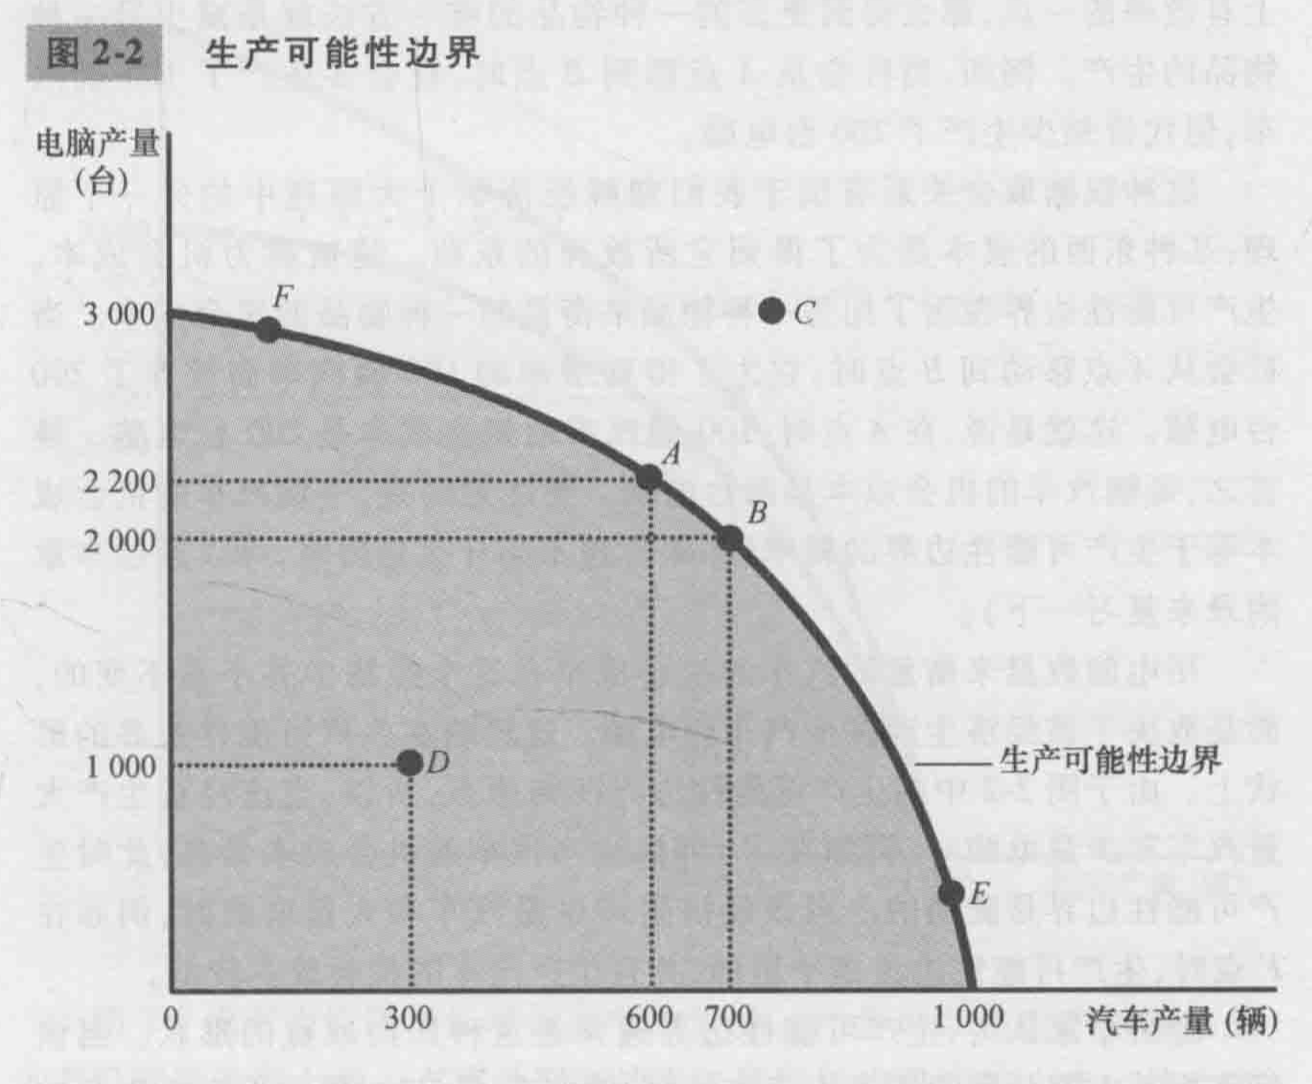
\includegraphics[width=8cm]{attachment/Fig2_2.png}
	\end{figure}
	从数学的视角来看, 两种产量$A_1,A_2$具有类似$A_1+A_2=C$的关系. 特别地, 极端追求汽车产量会让大量熟练于电脑生产的工人转而生产汽车, 这时付出很多电脑工人也只能推动汽车产量的微小变化, 因此越靠近$E$点, 一单位汽车所对应的电脑成本越高. 即是说整个曲线呈现上凸的形状. 
\end{example}

\subsection*{理性人考虑边际量}

实际上, 这个原理基于某种公设, 即所谓理性人(经济人)假设: \textit{人们总是以理性和利己的行为追求目标利益最大化}. 

用数学的话, 考虑一个将行为变成结果的函数$f$. 为了让$f(x)$取得最大值$M$, 可以先找到那些使得$f(x)$与$M$差距不大的$x$, 再在这些$x$(边际量)中找到$f(x)=M$的点. 

\begin{example}{沉没成本}
	已经付出且不可收回的成本, 就成为沉没成本. 按照边际分析的原理, 理性人不应当考虑沉没成本, 因为此时再付出多少都与沉没成本无关. (当然这是在不考虑个人情绪价值等的情况下)
\end{example}

\subsection*{人们会对激励做出反应}

在分析经济行为的后果时, 不仅要考虑其本身直接后果, 还要考虑其作为激励的影响. 

\begin{example}{关于弹性的直观认知}
	提高价格的确能增加生产者的单件收入, 但这会导致消费者的购买量减少, 总收益不一定增加. 注:实际上当需求弹性较小时收益会增加. 
\end{example}

\subsection*{比较优势原理: 贸易可以使每个人的状况都变得更好}

当贸易的两者各具有一方面的特长时, 贸易的优势是显然的. 实际上, 当其中一者具有绝对性优势时, 贸易也会带来改善. 





因此, 贸易可以让每个人都从事自己最擅长的活动. 


















% Appendices section.
% \appendix

% Include the "about" appendix from the BackMatter subfolder.
% \chapter{About the Authors}

\section{First Author}

\blindtext

\section{Second Author}

\blindtext

% Include the "abbreviation" appendix from the BackMatter subfolder.
% \chapter{Abbreviations}

\blindtext

% Include the "notation" appendix from the BackMatter subfolder.
% \chapter{Notation}

\blindtext

% Include the "code" appendix from the BackMatter subfolder.
% \chapter{Supplementary Scripts}

\blindtext

% Include the "glossary" appendix from the BackMatter subfolder.
% \chapter{Glossary}

\blindtext

% Include the "index" appendix from the BackMatter subfolder.
% \chapter{Index}

\blindtext

% Include the "references" appendix from the BackMatter subfolder.
% \bibliography{references.bib}
\bibliographystyle{ieeetr}
\nocite{*}

% End the document.
\end{document}
